\section{Introduction}
\label{sec:intro}

A useful accident anticipation system is not the one that predicts
\emph{that} an accident will happen.
It is the one that warns \emph{early enough to matter}, and explains
\emph{why that warning should be trusted}.
These two requirements---timeliness and interpretability---are central to
accident anticipation, yet existing work rarely treats
both as first-class objectives.
Most methods optimise classification accuracy only; almost all of them
remain black boxes.
For safety-critical deployment, this remains a substantial mismatch.
A system that cannot explain why it is dangerous, or provide a defensible
account of when it should warn, is harder to audit, calibrate, and deploy
responsibly in ADAS and autonomous driving pipelines~\citep{who2023global}.

\begin{figure*}[t]
  \centering
  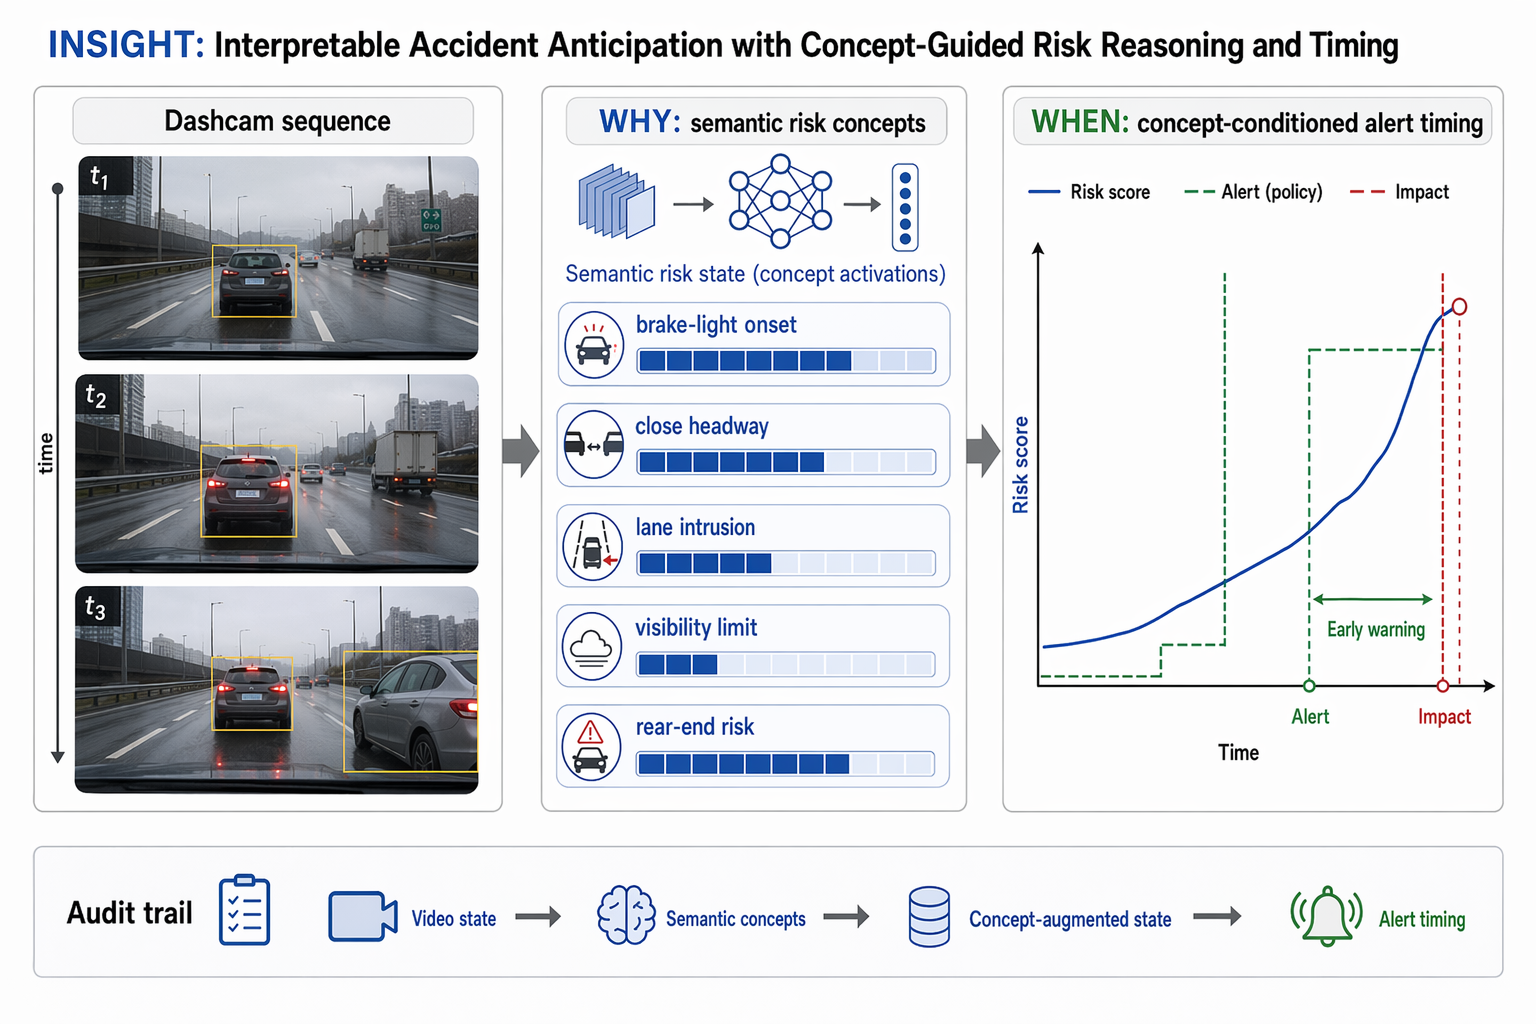
\includegraphics[width=0.985\textwidth]{../figures/insight_gpt_image2_teaser.pdf}
  \caption{\textbf{Schematic overview of \method{}.}
  \method{} builds an interpretable semantic risk state from video evidence,
  exposes \emph{why} risk is increasing through named concepts, and conditions
  \emph{when} to warn on that concept-augmented state. The dashcam panels are
  illustrative rather than evaluation evidence; real DAD case studies are
  reported in Figure~\ref{fig:multi}. The figure illustrates the intended link
  between semantic evidence (WHY) and concept-conditioned alert timing (WHEN)
  without treating the actor branch as a fully validated policy-level claim.}
  \label{fig:motivation}
\end{figure*}


\paragraph{What the field gets wrong.}
The recent literature has made impressive progress on Average Precision.
CCAF-Net~\citep{liu2025ccaf} reports 81.3\% AP on DAD,
and LATTE~\citep{ZHANG2025103173} reaches 89.7\%.
But these gains obscure two unresolved problems.

\textbf{First, existing methods are accuracy-optimal but timing-agnostic.}
Accident anticipation is usually formulated as binary classification with
cross-entropy loss.
This objective rewards confidence near the accident moment, where visual
evidence is strongest.
As a result, it systematically favours \emph{late certainty} over
\emph{early utility}.
In other words, the standard training objective is misaligned with the
real-world goal: every second of advance warning matters far more than a
small increase in probability immediately before impact.
The field has therefore optimised the wrong quantity.

\textbf{Second, the field lacks intrinsic dual-layer interpretability.}
A deployment-ready anticipation system must answer two distinct questions:
\emph{WHY is the scene dangerous?} and \emph{WHEN should the alert fire?}
Prior work addresses this only partially.
DRIVE~\citep{ref2} appends Grad-CAM after prediction---a post-hoc heatmap,
not a structural explanation.
W3AL~\citep{liao2024and} uses an LLM to verbalise accident location,
which is linguistic localisation rather than concept-level risk reasoning.
CRASH, DSTA, DAA-GNN, CCAF-Net, and LATTE provide no intrinsic
interpretability at all.
Few existing methods jointly explain both risk semantics (WHY)
and alert timing (WHEN) within the model itself.

\paragraph{Our central insight.}
The field has treated timing and interpretability as separate issues, but both
arise from the same modelling choice: framing accident anticipation as
classification rather than as semantic risk reasoning plus sequential timing
control. Once the decision state is defined as
$\mathbf{s}_t=[\mathbf{h}_t\|\mathbf{c}_t]$, with $\mathbf{c}_t$ containing
human-readable risk concepts, alert timing becomes conditioned on explicit
semantic evidence rather than on an opaque latent state alone. This view also
makes concept construction part of the method: in accident anticipation, a
generic visual vocabulary is often too noisy, while a fully manual ontology is
hard to scale. We therefore pair concept-conditioned timing control with a
reproducible pipeline for constructing risk concepts themselves.

\paragraph{\method{}: concept-augmented MDP state for dual-layer transparency.}
We propose \method{} (\textbf{In}terpretable \textbf{S}afety-\textbf{G}uided
accident anti\textbf{ci}pation via concep\textbf{t} bott\textbf{le}neck and
concept-aware actor-critic), a framework that couples a concept bottleneck,
concept-conditioned temporal modelling, and a timing-aware policy with a
reproducible risk-concept construction pipeline. Concretely, the model combines
(i) a concept discovery and polishing pipeline, (ii) the \cbm{} WHY layer,
(iii) the global \crs{} ranking, (iv) \cgta{} for concept-linked temporal
attention, (v) \tsd{} for anticipatory representation learning, and
(vi) \caac{} for concept-conditioned timing control.

The result is a jointly trained framework that couples an interpretable WHY
layer with a concept-conditioned timing mechanism, while grounding its semantic
interface in a reproducible ontology-construction pipeline.

\paragraph{Contributions.}
\begin{itemize}[leftmargin=1.4em,topsep=2pt,itemsep=1pt]
  \item We reframe accident anticipation as a \emph{concept-conditioned sequential decision problem} rather than binary classification with post-hoc explanation.
  \item We introduce a reproducible multimodal risk-concept construction pipeline and show through matched ontology comparisons that ontology choice changes the AP--mTTA operating point on DAD and A3D.
  \item We propose \method{}, which places semantic concepts directly in the decision state and thereby couples interpretable risk evidence with timing control.
  \item We present intervention evidence showing that concept edits can perturb downstream warning behaviour, while keeping policy-level claims scoped to the evidence currently available.
  \item We obtain 93.40\% AP / 4.90s mTTA on A3D and 68.19\% AP on DAD with a 30M-parameter model.
\end{itemize}
